\section{Auswertung}
\label{sec:Auswertung}

Im folgenden werden die Messungen, dargestellt in \autoref{fig:kurve1} bis \autoref{fig:kurve4}, ausgewertet.
Dafür wird zunächst die mittlere freie Weglänge bestimmt.
Dann wird die Energieverteilung der beschleunigten Elektronen errechnet, indem die Bremsspannung variiert wird.
% Franck-hertz_Kurve?


\subsection{Die mittlere freie Weglänge}
Mit \autoref{eq:tbd} und \autoref{eq:tbd} wird die mittlere freie Weglänge der beschleunigten Elektronen,
die aus der Heizkathode herausgelöst werden, berechnet.
Ebenfalls wird das Verhältnis $a / \bar{\omega}$ bestimmt.
Die Ergebnisse der Rechnung sind in \autoref{tab:tabelle1} dargestellt.

\begin{table} [H]
  \centering
  \caption{Die mittlere freie Weglänge.}
  \label{tab:tabelle1}
  \begin{tabular}{c c c}
      \toprule
      Temperatur $T / \unit\kelvin$ & $\bar{\omega} / \unit\meter$ & $\frac{a}{\bar{\omega}}$ \\
      \midrule 
      298,35 & 0.538412049 & 0.01857314\\
      433,25 & 0.000411729 & 24.2877893\\
      448,55 & 0.000239611 & 41.7343021\\
      459,05 & 0.000168744 & 59.2613673\\
      \bottomrule
  \end{tabular}
\end{table}

\subsection{Differentielle Energieverteilung}
Nun werden die Messdaten der ersten beiden Messungen ausgewertet.
Dabei handelt es sich um \autoref{fig:kurve1} und \autoref{fig:kurve2}, wobei die Graphen von einem X-Y-Schreiber erstellt wurden.
Die Beschleunigungsspannung wird zunächst konstant mit $U_\text{B} = 11 \unit\V$ gewählt.

\subsubsection*{Messung bei 298,35 Grad Kelvin}
Um die Energieverteilung in Abhängigkeit der Spannung zu erhalten, wird das Verhältnis von $\frac{\increment y}{\increment x}$ gebildet.
Dabei kann $y$ in Skalenanteilen angegeben werden.
Als 1 Skalenanteil wird ein Kästchen des Millimeter Papiers gewählt.
Die Werte sind in \autoref{tab:tabelle2} angegeben, beziehungsweise in \autoref{fig:plot1} abgebildet.
Es lässt sich erkennen, dass die Steigung den größten Abfall bei $U_\text{B, eff} = 7.75 \unit\V$ hat.
Damit haben die meisten Elektronen eine Energie in Beschleunigungsrichtung von $E = 7.75 \unit\eV$.
Schließlich lässt sich noch das Kontaktpotential mit \autoref{tbf} zu
\begin{equation}
  K = U_\text{B} - U_\text{B, eff} = (11 - 7.75) \unit\V = 3.25 \unit\V
\end{equation}
angeben.
% \begin{table} [H]
%   \centering
%   \caption{Die mittlere freie Weglänge.}
%   \label{tab:tabelle2}
%   \begin{tabular}{c c c}
%       \toprule
%       $U / \unit\V$ & $\frac{y}{\text{Skt}_y}$ & $m  =\frac{y_{i+1} - y_{i}}{U_{i+1} - U_{i}}$ \\
%       \midrule 
%       0   & 15.8  &  -  \\
%       1   & 14.1  & -1.7\\
%       2   & 12.6  & -1.5\\
%       3   & 11.1  & -1.5\\
%       4   & 9.6   & -1.5\\
%       5   & 7.8   & -1.8\\
%       6   & 6     & -1.8\\
%       7   & 4     & -2. \\
%       7,5 & 2.8   & -2.4\\
%       7,75& 1,5   & -5.2\\
%       8   & 0.8   & -2.8\\
%       9   & 0.3   & -0.5\\
%       10  & 0.3   & 0.  \\
%       \bottomrule
%   \end{tabular}
% \end{table}

% \begin{figure}
%   \centering
%   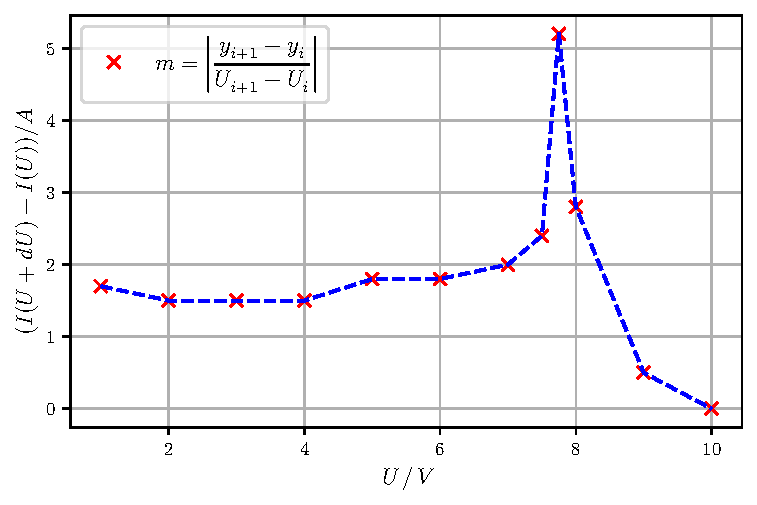
\includegraphics[width=0.5\linewidth]{build/plot1.pdf}
%   \caption{Die Steigung in Abhängigkeit der Spannung.}
% \end{figure}

\begin{table}[ht]
  \begin{minipage}[b]{0.4\linewidth}
  \centering
  \begin{tabular}{c c c}
    \toprule
    $U / \unit\V$ & $\frac{y}{\text{Skt}_y}$ & $m  =\frac{y_{i+1} - y_{i}}{U_{i+1} - U_{i}}$ \\
    \midrule 
    0   & 15.8  &  -  \\
    1   & 14.1  & -1.7\\
    2   & 12.6  & -1.5\\
    3   & 11.1  & -1.5\\
    4   & 9.6   & -1.5\\
    5   & 7.8   & -1.8\\
    6   & 6     & -1.8\\
    7   & 4     & -2. \\
    7,5 & 2.8   & -2.4\\
    7,75& 1,5   & -5.2\\
    8   & 0.8   & -2.8\\
    9   & 0.3   & -0.5\\
    10  & 0.3   & 0.  \\
    \bottomrule
  \end{tabular}
    \caption{Die gem. Messwerte bei 298,35 K.}
    \label{tab:tabelle2}
  \end{minipage}\hfill
  \begin{minipage}[b]{0.45\linewidth}
  \centering
  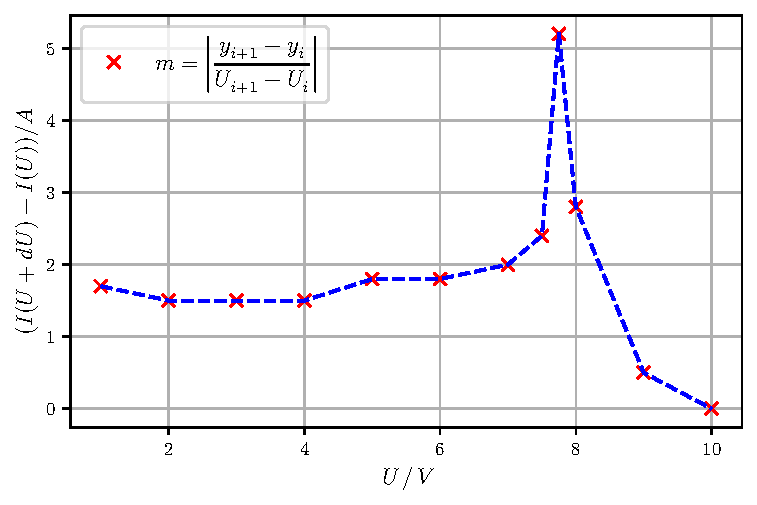
\includegraphics[width=\linewidth]{build/plot1.pdf}
  \captionof{figure}{Die Steigung in Abhängigkeit der Spannung.}
  \label{fig:plot1}
  \end{minipage}
\end{table}

\subsubsection*{Messung bei 433,25 Grad Kelvin}

Bei der Messung mit $433,25$ Grad Kelvin ergaben sich die Messwerte in \autoref{tab:tabelle3}.
Die Steigung wurde dann gegen die Bremsspannung in \autoref{fig:plot2} aufgetragen.
Auch hier lässt sich ein Maximum der Spannung direkt bei $U_{\text{B, eff}} = 1 \unit\V$ erkennen.

\begin{table}[ht]
  \begin{minipage}[b]{0.4\linewidth}
  \centering
  \begin{tabular}{c c c}
    \toprule
    $U / \unit\V$ & $\frac{y}{\text{Skt}_y}$ & $m  =\frac{y_{i+1} - y_{i}}{U_{i+1} - U_{i}}$ \\
    \midrule 
    0   & 17,8& - \\
    0,5 & 14,3& - 7 \\
    1   & 11  & -  6,6 \\ 
    1,5 & 8,3 & - 5,4 \\ 
    2   & 5,8 & - 5 \\  
    2,5 & 3,2 & - 5,2 \\ 
    3   & 1,4 & - 3,6 \\ 
    4   & 0,7 & - 0,7 \\
    5   & 0,7 & 0 \\  
    6   & 0,6 & - 0,1 \\ 
    7   & 0,6 & 0 \\ 
    8   & 0,5 & -  0,1 \\ 
    9   & 0,5 & 0 \\ 
    10  & 0,4 & -  0,1 \\
    \bottomrule
  \end{tabular}
    \caption{Die gem. Messwerte bei 433,25 K.}
    \label{tab:tabelle3}
  \end{minipage}\hfill
  \begin{minipage}[b]{0.45\linewidth}
  \centering
  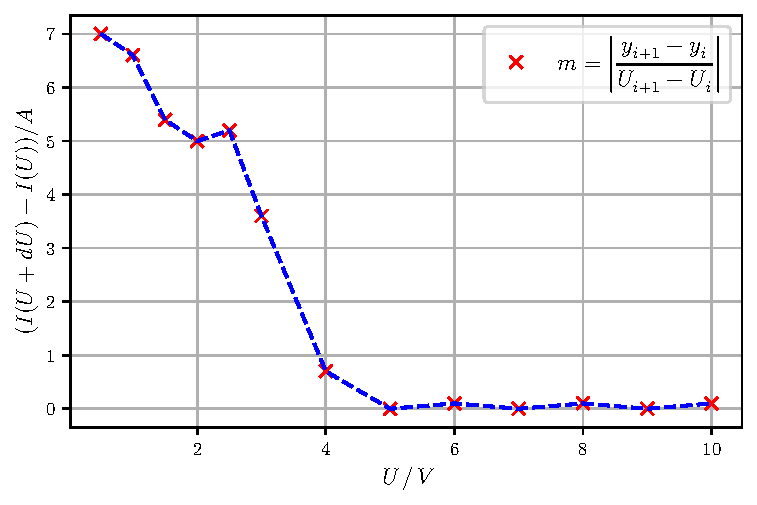
\includegraphics[width=\linewidth]{build/plot2.pdf}
  \captionof{figure}{Die Steigung in Abhängigkeit der Spannung.}
  \label{fig:plot2}
  \end{minipage}
\end{table}


\subsection{Auswertung der Franck-Hertz-Kurven}

Im folgenden werden die Messdaten aus \autoref{fig:kurve3} und \autoref{fig:kurve4} ausgewertet.
